Task B2 was to implement process handling in out operating system. Lets look a bit closer on the concept of processes before discussing the implementation.
\subsubsection{The process concept}
A process is a in an instance of a program (an executable) that runs in an operating system environment, 
and returns to this operating system upon completion. Hence, the operating system is the one resposible for 
creating new processes and terminating them. An analogy to this is the a java object, being an instance of a java class.\\
The process is therefore nothing more than a container for resources reserved to the process by the operating system. \\

\subsubsection{The thread concept}
A thread is the part of the process container responsible for executing the program. Usually processes can have a number of threads as iliustrated in figure \ref{fig:thread_models}.(a). \\

So, the operating system need to keep track of the running processes and take care of creating and terminating the processes. 
For this, we have added two system calls; create and terminate.

\begin{figure}
\centering
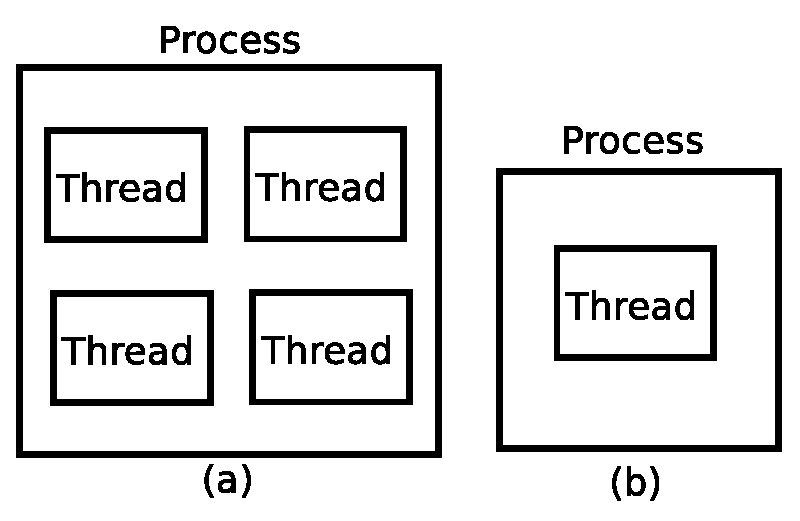
\epsfig{file=fig/Thread_Models.eps, height=1in}
\caption{Typical thread models}
\label{fig:thread_models}
\end{figure}

\subsubsection*{The create system call}
To implement this, we need to keep track of the running processes. This is handled by a process table that contains structures holding information about an individual process. \\
Processes are executed invoking this system call by executing a piece of assembler code that calls a named procedure called ``main'' and then calls terminate when main is done executing. In this system call we create one thread, and only one for each process, so our thread model actually looks like figure \ref{fig:thread_models}.(b)

\subsubsection*{The terminate system call}
When a program finishes the terminate system call is invoked. This does cleanup by of course cleaning up references to the process 
and the threads of the process, but also do a context switch. We switch back to the thread of the parent of the process just terminated.

\subsection{Reflections}

\subsubsection*{How is the system booted?}
Our virtual pc starts a BIOS that searches for a bootloader (in our case Grub), that then loads the kernel image to memory from a harddisk - or in our case a disk image. The virtual pc is an AMD64 architecture.

\subsubsection*{How are processes created from executable files?}
The kernel finds all executable files and loads them to memory, storing a pointer to the first instruction for each process. The function prepare\_process does a lot of sanity checks on the image assuring that it is in fact meant for execution.

\subsubsection*{How does a daemon (process) differ from processes studied in this task?}
Our processes runs ``interactively'' and daemons traditionally runs in the background. Otherwise they share the fact that they are started at bootup by the operating system.

\section{Test}
This task needs to have implemented the system calls ``createprocess'' and ``terminate'' so that the two executables are able to create process as stored in the executable\_table. After the executables have reached the end of their code they will make the system call to terminate. This desired result was achieved as defined in task definition, and the test was a success.